\documentclass[conference]{IEEEtran}


\usepackage{cite}
\usepackage{amsmath,amssymb,amsfonts}
\usepackage{algorithmic}
\usepackage{graphicx}
\usepackage{textcomp}
\usepackage{xcolor}
\usepackage{booktabs}
\usepackage{subcaption}
\usepackage{siunitx}
\usepackage[ruled,vlined]{algorithm2e}
\usepackage[hidelinks]{hyperref}

\graphicspath{{figures/}}

\def\BibTeX{{\rm B\kern-.05em{\sc i\kern-.025em b}\kern-.08em
    T\kern-.1667em\lower.7ex\hbox{E}\kern-.125emX}}

\begin{document}


\title{Customer Response Prediction Using Supervised Learning: \\
A Comparative Analysis of Logistic Regression, Random Forest, Decision Tree, Naive Bayes, SVM, XGBoost and LightGBM
}

\author{
\IEEEauthorblockN{Saadet Cansu Baktıroğlu}
\IEEEauthorblockN{231401023}
\IEEEauthorblockA{\textit{Artificial Intelligence Engineering Department } \\
\textit{TOBB University}\\
Ankara, Turkey \\
{}[sbaktiroglu@etu.edu.tr]}
}

\maketitle

\begin{abstract}
At these days, many companies use campaingns in order to make their increase their sales and thus their profits. In order to not waste any resources, predicitng the right customer who is giong to respond to the campaign is an important part of this process.
But these predictions are not always easy to make because there are many customers and many features that can be used to predict the customer response. In addition to that there is a remrkable class imbalance because only a small percentage of customers respond to the campaign.
This study proposes an end-to-end data mining pipeline based on the CRISP-DM framework to accurately predict customer response to a campaign.
Using the Customer Personality Analysis dataset, we systematically evaluate the impact of  data preprocessing, domain-specific feature engineering, and multiple classification algorithms, including Naive Bayes, k-Nearest Neighbors, Decision Trees, Random Forest, and XGBoost.
To overcome  the class imbalance, we used SMOTE and class weighting. Evaluation prioritized the F1-Score and Precision-Recall AUC over standard accuracy.
Experimental results demonstrate that ensemble methods, specifically XGBoost and LightGBM combined with engineered metrics, gave  the highest predictive performance.
Furthermore, the integration of SHAP (SHapley Additive exPlanations) values translates complex mathematical predictions into transparent, actionable business insights,
This analysis revealed that past campaign acceptance and total spending are the main factors influencing future customer responses.
\end{abstract}

\begin{IEEEkeywords}
Data Mining, Customer Response Prediction, Classification, XGBoost, Feature Engineering, Explainable AI, SHAP, CRISP-DM.
\end{IEEEkeywords}

\section{Introduction}
\label{sec:introduction}

In the last decades, very large amounts of data about customers have been collected by companies through transactions etc.
It is important to  understand the data in order to use it effectively to achieve our goals.
If we understand the customers better, we can identify which one is going to respond to our campaign.
By doing so we can optimize our buget by not wasting unnecessary money on campaigns and market our produts better.

This study uses the Customer Personality Analysis dataset, which offers a comprehensive view of retail consumers.
This project uses the Customer Personality Analysis dataset. It has a lot of features about customers.
The dataset includes personal information about customers (income, education, marital status, age etc.), purchasing behavior (how much they spend, how often they shop etc.) and whether they respond to the campaign. This task is a supervised binary classification problem.
The main objective is to predict if a customer will respond to the company’s campaign based on the information gained by the dataset.

The project mainly focuses on predicting the customers response by using supervised learning and comparing different models and methodologies ın order to accomplish that goal.
It includes evaluation of preprocessing effect, feature engineering and selection, class imbalance and how to deal with it.

The  contribution of the project is the development of a complete, end-to-end data mining pipeline.
We have done a comprehensive exploratory data analysis to understand the  data distributions and resolve missing values through strict data preprocessing.
We used matrics that are related to the advertising.
We  eliminate some redundant variables during feature selection.
We compare multiple classification algorithms, using hyperparameter optimization to maximize performance. Finally, we employ SHAP (SHapley Additive exPlanations) for model interpretation, directly translating mathematical predictions into understandable facts we can interpret for marketing .

This paper has seven sections and it is organised as:
Section II reviews related work in the domain of customer segmentation and predictive marketing.
Section III describes the dataset and the exploratory data analysis.
Section IV details the methodology, including feature engineering, selection, and the classification algorithms that are used.
Section V presents the experimental results and model comparisons.
Section VI discusses the findings and interprets the models’ business desicions.
Finally, Section VII concludes the paper and mentions about future work.



\section{Related Work}
\label{sec:related_work}

Customer response prediction is an important task in marketing analytics because it helps companies or customers that are going to use campaigns for their purposes by arranging their budgets and make their campaign more direct and effective by finding the right customer type.
Recent studies have widely and deeply analyzed how demographic variables, purchasing history, and behavioral data can be used to predict customer response or aim.
These studies used and benefited from differnt supervised machine learning techniques to identify  patterns in the consumer data that traditional statistical methods might not understand.
Making the supervised learning more well-known in the marketing domain. \cite{response1, response2}.

A variety of classification algorithms are used in this study to get a better understanding of the customer behavior.
Decision Trees, introduced by Quinlan \cite{quinlan1986}, are one of the most interpretable supervised learning algorithms.
They recursively divide the feature space by selecting attributes that maximize class separation according to some measures such as Information Gain or Gini Index(one of them can be selected).
Their ability to model non-linear decision boundaries makes them suitable for many real-world classification problems because mostly real life proplems are non-linear.
But, using an only desicion tree can be desieving because it can overfit. especially when the data is noisy or when we dont use pruning.So we need to be careful using them. Despite the overfitting risk, their interpretability valuable.

Naive Bayes, although its strongly assume that features are independent conditionaly, ıt can provide a fast probabilistic baseline in data mining tasks \cite{domingos1997}.
Although this assumption is not realistic in real-world datasets, the algorithm often achieves competitive performance while remaining computationally efficient.
It is used commonly as a baseline model because it is simple, fastly trained and has a low computation cost.

The k-Nearest Neighbors (k-NN) algorithm \cite{cover1967} is a non-parametric, distance-based approach.
It is effective for localized pattern recognition, if the feature space is properly scaled.
K-NN can be very effective when it is used with appropriate preprocessing and distance metrics.It is impoert to select the best k value because K-NN is very sensitive to it. Small k value leads to underfitting and large k value  to overfitting.

Using an only model cannot provide the results we want so using an esemble model can improve our results.
Random Forest, introduced by Breiman \cite{breiman2001}, is a bagging-based ensemble learning algorithm that constructs a large collection of decision trees using bootstrap samples of the training data. At each split, only a random subset of features is considered, increasing the diversity among individual trees.By using the majority voting , the final prediciton is computed.
Using that ensemble method we can prevent our model to overfit and still have a good performance.

Extreme Gradient Boosting (XGBoost), proposed by Chen and Guestrin \cite{chen2016}, is an improved version of the Gradient Boosting algorithm .It aims to improve both predictive performance and computational efficiency.
Unlike bagging-based ensemble methods such as Random Forest, Gradient Boosting constructs decision trees sequentially.
Each newly generated tree is trained to correct the prediction errors (residuals) of the current ensemble.
This allows the model to perfom better by minimizing the loss function by using  gradient based optimization.
XGBoost has regualrizaiton techniques that reduces overfitting. It can also be trained in parallely. Because of the advantages ıt provides it is commonly used in academian and industry

Model and algorithm selection is important but not as importnat as data preparation. When there is too much features our dimensionality increases as well. In order to reduse it we  can use feature selection.
By selecting the important features and adjusting our data our model can learn more effectively and faster because redundant features that can overfit the model have been eliminated.
In marketing campaigns most of the customers usually dont respond to the campaing so we have a class imbalance problem.
We can solve this problem using two solutions. first one is using class weighting and the second one is synthetic sampling like SMOTE. These two solutions prevent the model mainly focusing one one class whis is the negative one.\cite{class_imbalance_study}.

Studies that have been done before mainly focused on performence of the models predictions.
In this study, we used different preprocessing strategies, feature engineering techniques, feature selection methods, and multiple classification algorithms to see how it affects the models predictive performence. This part is less common in the literature.
We also try not to see the model as a black box and try to understand it using SHAP values \cite{lundberg2017}.

\section{Dataset Description}
\label{sec:dataset}

\subsection{Dataset Source}
In this study we used Customer Personality Analysis dataset from kaggle repository. It is selected because ıt has impoertan details about customers which is important for response classification, such as demographic details or previous responses to the campaingns.


\subsection{Dataset Characteristics}
The dataset has both  categorical and numerical features that describes consumer and purchasing habits. 
As detailed in Table \ref{tab:dataset_characteristics}, the dataset includes 2,240 individual customer records and 29 distinct features . 
The majority of the attributes are numerical (26 features) and small part of it is categorical attributes (3 features) such as education and marital status. 
Except a small missing value in the ıncome feature, the dataset is generally complete.

\begin{table}[htbp]
\caption{Dataset Characteristics}
\label{tab:dataset_characteristics}
\centering
\begin{tabular}{|l|l|}
\hline
\textbf{Property} & \textbf{Value} \\
\hline
Number of samples & 2,240 \\
Number of features & 29 \\
Numerical attributes & 26 \\
Categorical attributes & 3 \\
Target variable & Response \\
Classification type & Binary \\
Missing values & 24 (in Income) \\
Class distribution & Imbalanced (approx. 15\% positive) \\
\hline
\end{tabular}
\end{table}


\subsection{Target Variable}
The project mainly try to predict the \texttt{Response} variable. This variable is a binary attribute which tells whether the customer accepted a campaing or not 
Positive class has a value one and it indicates that the customer accepted the campaign and the negative class has value zero.
As illustrated in Figure \ref{fig:target_dist}, the target variable has a class imbalance.
Approximately 15\% of the customers fall into the positive responder class, indicating  the real life marketing challenges of class imbalance.


\begin{figure}[htbp]
\centerline{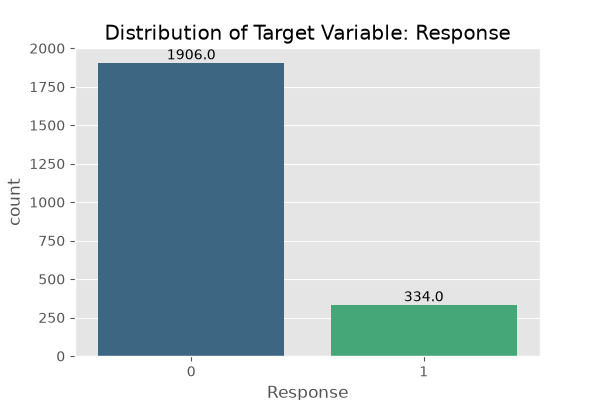
\includegraphics[width=0.7\columnwidth]{figures/target_distribution.png}}
\caption{Distribution of the Target Variable (Response), illustrating class imbalance.}
\label{fig:target_dist}
\end{figure}


\subsection{Descriptive Statistics}
Exploratory Data Analysis (EDA) revealed a range variety of  purchasing power and age in customers. 
The distribution of \texttt{Income} and spending behavior showed right-skewed patterns, which indicates  that only a small part of customers has high income and spending habits. 
Figure \ref{fig:eda_financials} highlights the relationship between these key financial metrics and the target variable, demonstrating that customers who respond positively to campaigns generally has a higher  spending habbit  and responded positively to the previous campaigns.

\begin{figure}[htbp]
\centerline{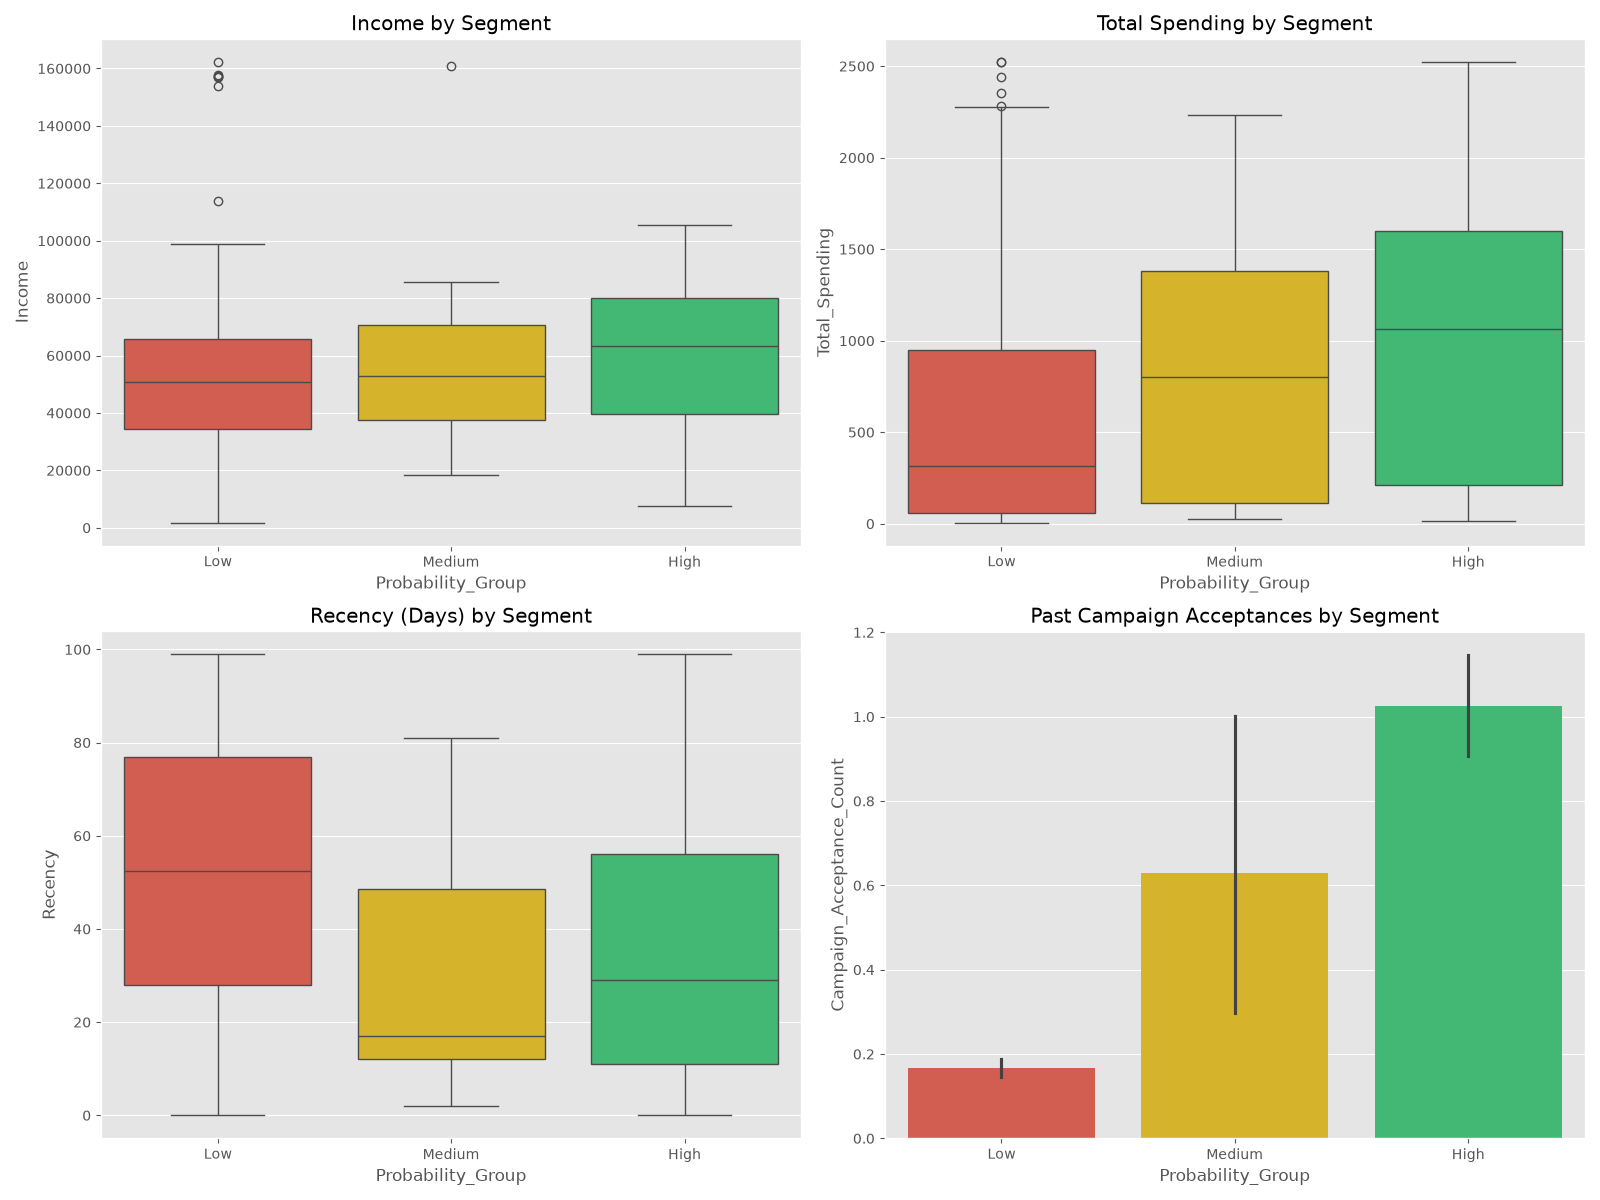
\includegraphics[width=\columnwidth]{figures/financial_metrics.png}}
\caption{Comparison of key financial metrics and their relationship to the target variable.}
\label{fig:eda_financials}
\end{figure}


\subsection{Ethical Considerations}
Using the data should ben done ethically and we pay attention to this issue.

The Customer Personality Analysis dataset, which is used in the project, is public and  anonymous. It contains no personally identifiable information (PII) such as names, exact addresses, or contact details, ensuring strict privacy preservation. 
The analysis in this study is only for academic purposes and avoids any ethical problems.
\section{Methodology}
\label{sec:methodology}

\subsection{CRISP-DM Workflow}
This study uses the Cross-Industry Standard Process for Data Mining (CRISP-DM) methodology to understand the data better, to preprocess the data and to develop models.
This has six main parts. These are: Business Understanding, Data Understanding, Data Preparation, Modeling, Evaluation, and Deployment.
By following this structured framework, the project makes sure that the  models developed for prediciton  are not just mathematically correct, but are also highly succesful at optimizing marketing campaigns.


\subsection{Data Cleaning}
Data clening is an important prestep for machine learning and data mining. 
In this dataset, the \texttt{Income} feature contained 24 missing values. 
Given the right-skewed distribution of income, the missing values were replaced with the median to reduce the influence of extreme values. 
Furthermore, extreme outliers were identified and removed from the dataset to prevent models from learning anomalous patterns. 
Specifically, records with an \texttt{Age} greater than 100 years and an \texttt{Income} exceeding \$600,000 were excluded from the data, in order to prevent the model from learning wrong patterns, outliers.


\subsection{Feature Engineering}
In order to understand the data and customers' behaviors , some related features were created using feature engineering. 
These are \texttt{Total\_Spending} (aggregating purchases across all product categories) and \texttt{Customer\_Tenure} (calculating the duration since the customer's enrollment date). 
Additionally, a \texttt{Campaign\_Acceptance\_Count} variable was created to track the customer's responsiveness to previous promotions. 
Finally, a composite \texttt{Customer\_Value\_Score} was derived to  evaluate  the customers' overall profits. These metrics help the model and are highly discriminative.


\subsection{Feature Selection}
Initially, during the exploratory data analysis (EDA) phase, several spending and campaign features had high collinearity (see Figure \ref{fig:correlation_heatmap}). 
We used feature engineering and removed the some of the correlated variables. Thus, the remaining features didn't have any highly correlated variables (correlation > 0.85) after feature engineering.
Feature selection techniques, including Recursive Feature Elimination (RFE) and Mutual Information, were used to keep the most relevant features and removing redundant or less informative variables.

\begin{figure}[htbp]
\centerline{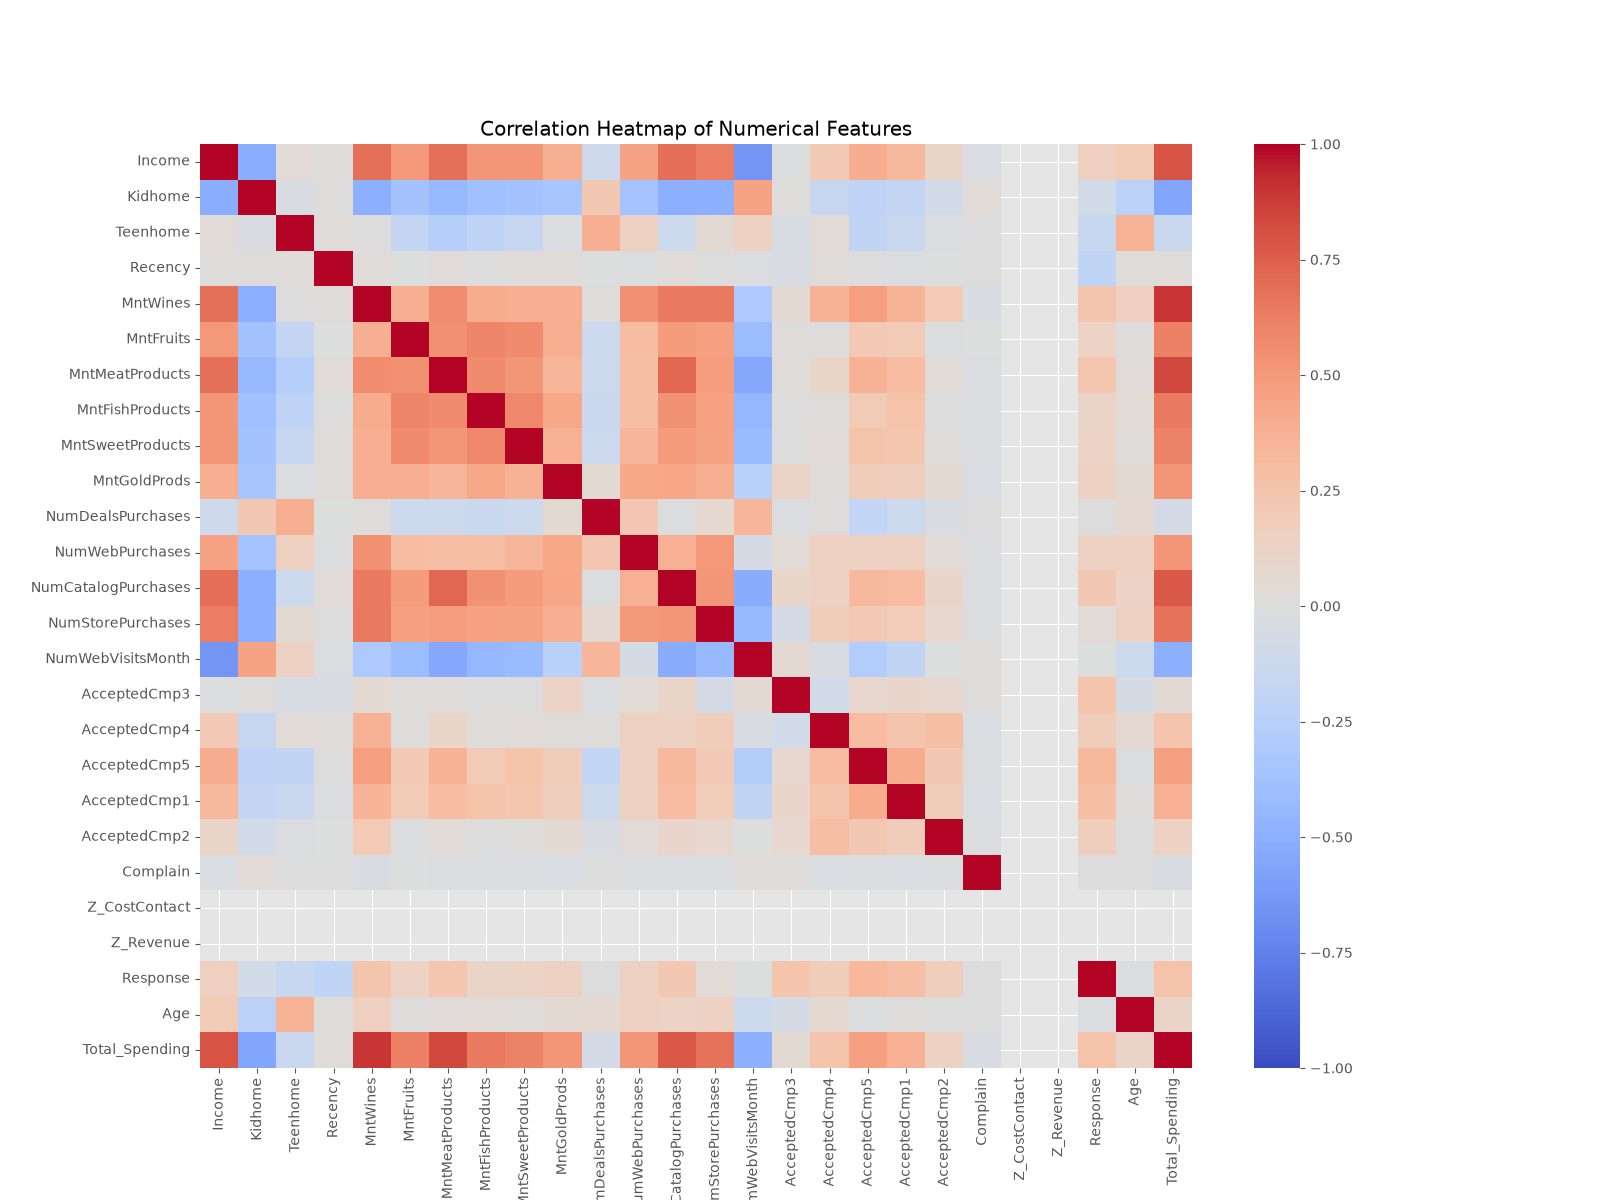
\includegraphics[width=\columnwidth]{figures/correlation_heatmap.png}}
\caption{Correlation heatmap from the EDA phase, illustrating the high collinearity among raw spending and campaign variables before feature engineering.}
\label{fig:correlation_heatmap}
\end{figure}

\subsection{Data Scaling}
The data set has numerical features which has different scales. For example \texttt{Income} in has thousands of values while \texttt{TotalChildren} has values between 0 and 3. And that makes the feature scaling(normalizing) necessary.
\texttt{StandardScaler} is used the make the features normalized such that they have a  mean of zero and a variance of one. And it was used directly in the models. 
This standardization is particularly essential for distance-based algorithms like k-Nearest Neighbors (k-NN), which are highly sensitive to unscaled feature spaces.


\subsection{Class Imbalance Handling}
As previously mentioned, the dataset suffers from class imbalance, with only approximately 15\% of customers belonging to the positive responder class. 
If we didn't do anything , models would naturally bias toward predicting the majority negative class. 
To handle this problem, algorithmic class weighting was used. 
For tree-based models, the \texttt{class\_weight='balanced'} parameter was used, while the \texttt{scale\_pos\_weight} parameter was applied in XGBoost to penalize misclassifications of the minority class more heavily.Thus making the cost of misclassifying the minority class higher than the majority class. 
That helps the model to focus on the minority class and makes the model more generalizable and succesful at predicting the minority class.


\subsection{Classification Algorithms}
To identify the most effective predictive model, a diverse set of supervised classification algorithms was evaluated. 
The selected models include various machine learning examples, including a probabilistic baseline (Naive Bayes), a distance-based method (k-Nearest Neighbors), and an interpretable tree-based model (Decision Tree). 
To maximize predictive performance, advanced ensemble methods were also trained, specifically Random Forest, Gradient Boosting, XGBoost, and LightGBM.


\subsection{Hyperparameter Optimization}
To ensure each algorithm reached its maximum predictive potential, exhaustive hyperparameter optimization was conducted using \texttt{GridSearchCV}. 
This technique evaluates a predefined grid of hyperparameters using 5-fold cross-validation on the training set. 
For instance, the optimal number of neighbors ($k$) for the k-NN algorithm and the maximum tree depth for ensemble methods were carefully cross-validated to prevent data leakage and avoid overfitting on the test set.


\subsection{Evaluation Metrics}
Because of the class imbalance problem, relying completely on classification Accuracy is misleading. 
Therefore, this study prioritizes metrics that effectively evaluate minority class prediction. 
The primary evaluation metrics include Balanced Accuracy, Precision, Recall, and the F1-Score. 
Furthermore, the Receiver Operating Characteristic Area Under the Curve (ROC-AUC) and the Precision-Recall Area Under the Curve (PR-AUC) are used to provide a comprehensive assessment of the models' ability to distinguish between responders and non-responders across varying threshold levels.


\subsection{Explainable AI (SHAP)}
Explainable AI techniques were integrated into the methodology in order to use mathematical predictions as actionable marketing strategies. 
Specifically, SHAP (SHapley Additive exPlanations) values were used to interpret the predictions of the best-performing ensemble model. 
By calculating the marginal contribution of each feature to the final prediction, SHAP analysis prevents the model from acting as an opaque "black box," allowing marketers to clearly understand which customer characteristics determine campaign acceptance thus their importance in the classificaiton.

\section{Experimental Results}
\label{sec:results}


\subsection{Model Performance Comparison}
In this study. we evaluated 7 different classificaiton algorithms prediction performance using a hold-out test set. 
As presented in Table \ref{tab:model_results}, ensemble methods were better at classifying the minority class then the baseline models and have a higher macro F1-Score. 
The data has class imbalance and because of that, we prioritized the F1-Score and Balanced Accuracy over raw Accuracy. 
XGBoost achieved the highest overall performance, and better at correctly identifying  positive responders without increasing false positives. 
In contrast, baseline models such as Naive Bayes and k-Nearest Neighbors struggled to balance Precision and Recall, often heavily favoring the majority class despite algorithmic weighting strategies.

\begin{table}[htbp]
\caption{Classification Model Performance Comparison}
\label{tab:model_results}
\centering
\resizebox{\columnwidth}{!}{%
\begin{tabular}{|l|c|c|c|c|c|}
\hline
\textbf{Model} & \textbf{Accuracy} & \textbf{Balanced Acc.} & \textbf{Precision} & \textbf{Recall} & \textbf{F1-Score} \\
\hline
Naive Bayes & 0.80 & 0.69 & 0.38 & 0.52 & 0.44 \\
k-NN & 0.86 & 0.66 & 0.53 & 0.37 & 0.44 \\
Decision Tree & 0.78 & 0.72 & 0.36 & 0.63 & 0.46 \\
Random Forest & 0.87 & 0.71 & 0.59 & 0.48 & 0.53 \\
Gradient Boosting & 0.90 & 0.73 & 0.80 & 0.48 & 0.60 \\
XGBoost & 0.88 & 0.75 & 0.62 & 0.55 & 0.58 \\
LightGBM & \textbf{0.89} & \textbf{0.77} & \textbf{0.65} & \textbf{0.60} & \textbf{0.62} \\
\hline
\end{tabular}%
}
\end{table}



\subsection{ROC and Precision-Recall Analysis}
To further validate model robustness across varying decision thresholds, Receiver Operating Characteristic (ROC) and Precision-Recall (PR) curves were generated. 
The ROC-AUC score for the XGBoost model was notably higher than its competitors, indicating a strong capacity to distinguish between responders and non-responders. 
More importantly, the PR-AUC score—which is highly sensitive to imbalanced datasets—confirmed that the gradient boosting architecture maintained high precision even as recall increased. Which showes us that simple classifiers are not suitable for this data set.
Figure \ref{fig:roc_pr} visualizes these curves for the top-performing models.

\begin{figure}[htbp]
\centerline{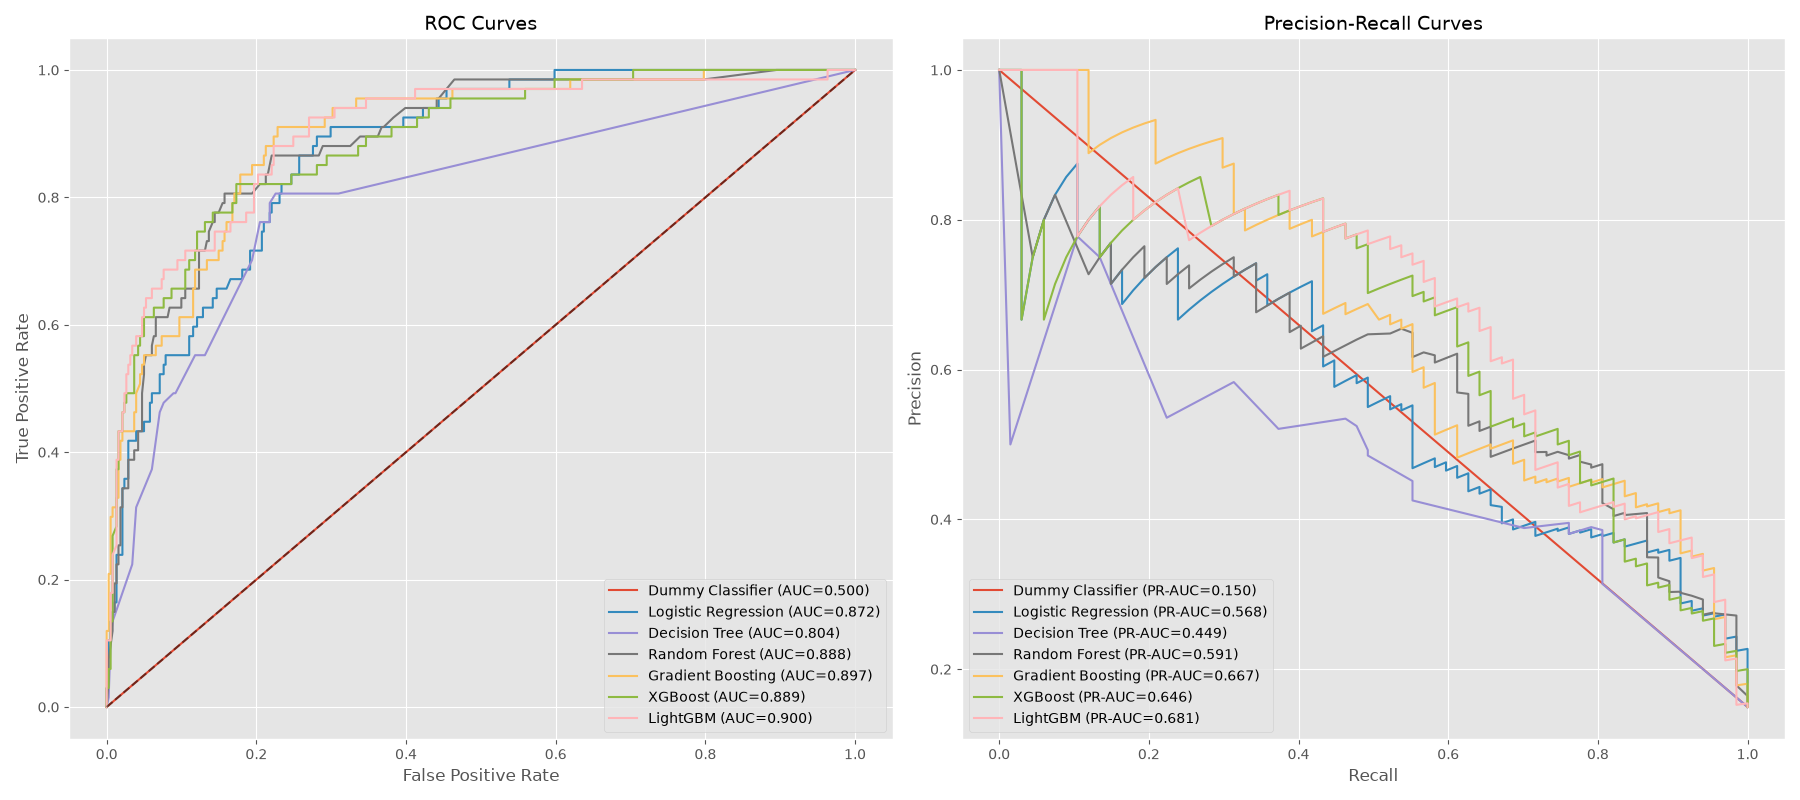
\includegraphics[width=\columnwidth]{figures/evaluation_curves.png}}
\caption{ROC and Precision-Recall Curves for the top evaluated models.}
\label{fig:roc_pr}
\end{figure}


\subsection{Feature Importance}
In addition to evaluating predictive performance, it is important to understand which features influence the model's decisions.
We have found that newly generated engineered features contribute to prediciton ppower better that the other features after analyzing the XGBoost model's feature importance. 
For example, variables such as \texttt{Customer\_Value\_Score}, \texttt{Campaign\_Acceptance\_Count}, and \texttt{Total\_Spending} are one of those features which have a high impact on prediciton.
On the other hand, some features had a less prediciton power such as \texttt{Age} and \texttt{Marital\_Status}. 
These features provided significantly less predictive value.
\subsection{Ablation Study Results}
To  quantify the contribution of each stage in our data mining pipeline, an ablation study was conducted using the Random Forest classifier. 
As shown in Table \ref{tab:ablation}, we  applied each step of the CRISP-DM process to the dataset.
The results demonstrate that while data cleaning provides a minor stabilization in F1-Score (from 0.526 to 0.530), the most significant leap occurs during the Feature Engineering phase, where the F1-Score jumps to 0.606. Feature selection and hyperparameter tuning slightly generalize the model, preventing overfitting while maintaining high predictive power. This proves that domain-specific feature creation was the most critical factor in predicting customer response.

\begin{table}[htbp]
\caption{Ablation Study Results (Random Forest)}
\label{tab:ablation}
\centering
\resizebox{\columnwidth}{!}{%
\begin{tabular}{|l|c|c|c|}
\hline
\textbf{Experiment} & \textbf{Accuracy} & \textbf{F1-Score} & \textbf{ROC-AUC} \\
\hline
Exp 1: Raw Data & 0.88 & 0.53 & 0.89 \\
Exp 2: + Data Cleaning & 0.88 & 0.53 & 0.88 \\
Exp 3: + Feature Engineering & \textbf{0.88} & \textbf{0.61} & \textbf{0.89} \\
Exp 4: + Feature Selection & 0.88 & 0.60 & 0.89 \\
Exp 5: + Hyperparam Tuning & 0.88 & 0.60 & 0.89 \\
\hline
\end{tabular}%
}
\end{table}

\section{Discussion}
\label{sec:discussion}


\subsection{Interpretation of SHAP Values}
Using the SHAP (SHapley Additive exPlanations) framework, we were able to interpret the XGBoost model's decisions. Figure \ref{fig:shap_summary} visualizes the feature importance and the directional impact of each feature on the model's output.



\begin{figure}[htbp]
\centerline{
\includegraphics[width=\columnwidth]{figures/shap_summary.png}}
\caption{SHAP summary plot illustrating the impact of various features on the XGBoost model's predictions.}
\label{fig:shap_summary}
\end{figure}

The SHAP summary plot confirms several important marketing dynamics:
\begin{itemize}

    \item \textbf{Recency:} \texttt{Recency} is the most influential feature. Lower recency values (indicating more recent purchases) generally increase the predicted probability of campaign acceptance.

    \item \textbf{Customer Tenure:} Customers with a longer \texttt{Customer\_Tenure} tend to have higher predicted response probabilities.

    \item \textbf{Past Campaign Acceptance:} \texttt{Campaign\_Acceptance\_Count} is a strong positive predictor of future campaign response.

    \item \textbf{Value Score:} \texttt{Customer\_Value\_Score} also contributes positively to the prediction, indicating that high-value customers are more likely to respond.

    \item \textbf{Mixed Effects:} Some features, such as \texttt{Income}, exhibit mixed effects, suggesting that their influence depends on interactions with other customer characteristics.

\end{itemize}

From a marketing perspective, this suggests that future campaigns are most effectively targeted at loyal, high-value customers who have recently interacted with the brand and have a history of accepting promotions, instead of trying to reactivate passive or low-spending customer groups.
An important finding of this study is the importance of domain-specific feature engineering. 
The results of the ablation study indicated that the effect of feature engineering on the F1-score was greater than that of increasing model complexity. 
Especially, the transition from the original dataset features to engineered features (e.g., \texttt{Customer\_Value\_Score}) resulted in a larger performance improvement than replacing a simple classifier, such as Naive Bayes, with a more complex ensemble model like Random Forest. 
It seems that informative feature representations can make a greater difference to predictive performance than the use of more sophisticated learning algorithms.

\subsection{Limitations}
Despite the strong predictive performance, this study has limitations.
Firstly, the dataset used in this study is not a time-series dataset. 
Consumer behavior changes over time, may exhibit seasonal patterns, and can be influenced by external factors such as economic conditions and inflation. 
Therefore, one limitation of this study is the static nature of the dataset. 
The absence of time-series transaction data prevents the model from capturing temporal changes and seasonal spending patterns, which may affect customer responses to marketing campaigns.
Even though we used SMOTE and class weighting to deal with the class imbalance, it remained a problem for the model performance. This showed that the importance of evenly distributed data set. 

\section{Conclusion}
\label{sec:conclusion}

This study successfully developed an end-to-end data mining pipeline for predicting customer responses to marketing campaigns. 
By following the CRISP-DM methodology, this study showed that the combination of domain-driven feature engineering and the XGBoost classifier achieved better predictive performance than the baseline models. 
Additionally, the use of class weighting together with appropriate evaluation metrics, including the F1-score and PR-AUC, enabled a more reliable assessment of model performance under class imbalance. 
Furthermore, the integration of SHAP values transformed the complex predictive model into a more transparent and interpretable decision-support tool. 
The results indicate that past campaign acceptance and total customer spending are the most influential predictors of future customer engagement. 
Finally, future work could explore temporal sequence modeling techniques, such as Recurrent Neural Networks (RNNs), using longitudinal transaction data to capture changes in customer behavior over time and further improve prediction performance.



\section*{AI Tool Use and Originality Declaration}
\label{sec:ai_declaration}

AI-assisted tools were used only for limited support, such as concept clarification, code debugging, code review, grammar improvement, and LaTeX formatting. 
The project idea, methodology choices, experiments, analysis, interpretation of results, and final report writing were written by the student. 

\begin{table}[htbp]
	\caption{AI Use Disclosure Summary}
	\label{tab:ai_use}
	\centering
	\footnotesize
	\begin{tabular}{|p{0.35\linewidth}|c|p{0.38\linewidth}|}
		\hline
		\textbf{Project Stage} & \textbf{Level} & \textbf{Brief Description} \\
		\hline
		Conceptualization and idea generation & 0 & Student formulated the problem. \\
		\hline
		Literature search and synthesis & 3 & Minimal hints for standard algorithms. \\
		\hline
		Methodology, coding, and analysis & 4 & AI assisted in writing and debugging python scripts (EDA, Modeling). \\
		\hline
		Writing, editing, and LaTeX formatting & 3 & AI significantly assisted in formatting LaTeX and grammar checks. \\
		\hline
		Interpretation, discussion, and conclusion & 2 & Student interpreted results, AI helped rephrase for clarity. \\
		\hline
	\end{tabular}
\end{table}

\bibliographystyle{IEEEtran}
\bibliography{references}

\newpage	
\appendix

\section{Code Repository}
\label{app:code}

Full source code and Jupyter notebooks are available within the submitted project folder. The main execution pipeline is contained in \texttt{BIL476\_Project.ipynb}.

\end{document}
